\section{What a Thorin computation sees at positive time}\label{cp:sec:see}

The P\'olya route computes $\xi_t$ at the cost of $\xi$, since the flow only reweights the kernel (Section~\ref{sec:ch21:flow}), and, when $(t,\alpha)\in\mathcal G$, the Thorin density of the shifted time $t$ clock is $\pi^{-1}v_t(\alpha,\theta)$ with
\[\begin{gathered}
v_t(\alpha,\theta)=\re\frac{\xi_t'}{\xi_t}(\alpha+i\theta),\\
\xi_t(s)=8\int_0^\infty e^{tu^2}\Phi_{\rm dBN}(u)\cosh(2wu)\,du,\\
\xi_t'(s)=8\int_0^\infty e^{tu^2}\Phi_{\rm dBN}(u)\,2u\sinh(2wu)\,du,
\end{gathered}\]
$w=s-\frac12$, by Remark~\ref{cp:rem:transfer}; where membership in $\mathcal G$ is not known, as at $t=0$ with $\alpha=0.6$, the function $v_t/\pi$ is still defined. We computed $v_t(\alpha,\theta)$ at the two times $t=0$ and $t=0.2$ and the two basepoints $\alpha=0.6$ and $0.75$, for $0\le\theta\le100$ in steps of $0.25$, with no primes and no list of zeros. The integrals were evaluated by the trapezoid rule of Section~\ref{sec:ch4:trapezoid} with step $1/160$ on $[0,1.6]$ (the tail beyond $1.6$ is below $10^{-812}$) at $\lfloor0.36\,\theta\rfloor+35$ digits, the term $0.36\,\theta$ absorbing the cancellation $|\xi_t(\alpha+i\theta)|\approx e^{-\pi\theta/4}$ that the P\'olya route always carries (Section~\ref{ch:polya}). A second discretisation, with step $1/125$ on $[0,1.9]$ and $15$ more digits, agrees with the first in $v_t$ at all $1604$ points of the four grids to a relative $2\times10^{-35}$; at $t=0$ the integrals, evaluated with $10$ more digits, agree with the closed forms of $\xi$ and $\xi'/\xi$ through $\Gamma$, $\psi$, $\zeta$ and $\zeta'$ to at least $43$ digits at both basepoints and at $\theta=0$, $17.5$, $50$ and $100$, and at $t=0.2$ the integral for $\xi_t'$ agrees with a central difference of $\xi_t$ to $30$ digits at two points.

\begin{figure}[ht]
\centering
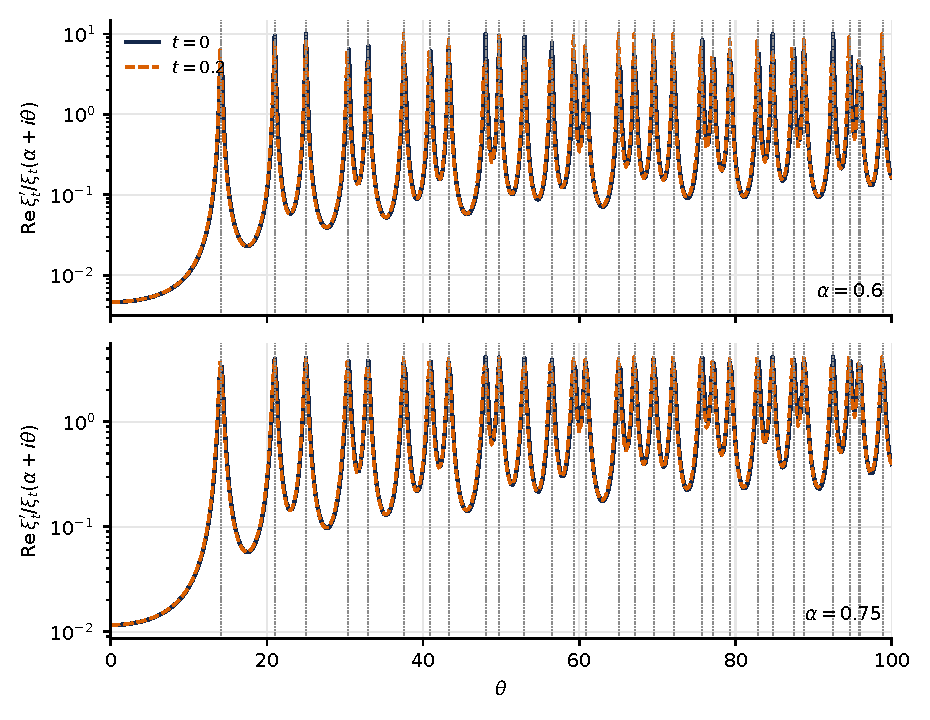
\includegraphics[width=0.88\textwidth]{fig/cp_thorin_t.pdf}
\caption{$v_t(\alpha,\theta)=\re\,\xi_t'/\xi_t(\alpha+i\theta)$, which is $\pi$ times the Thorin density of the shifted time $t$ clock when $(t,\alpha)\in\mathcal G$, on the lines $\re s=0.6$ and $0.75$, at $t=0$ (solid) and $t=0.2$ (dashed), from the P\'olya integral. Dotted lines mark the ordinates of the zeros of $\zeta$. Script \texttt{phase\_thorin.py}.}
\label{cp:fig:thorint}
\end{figure}

\begin{table}[ht]
\centering\small
\begin{tabular}{@{}rrrrrrr@{}}
\toprule
 & \multicolumn{3}{c}{$\alpha=0.6$} & \multicolumn{3}{c}{$\alpha=0.75$}\\
$\theta$ & $t=0$ & $t=0.2$ & change & $t=0$ & $t=0.2$ & change\\
\midrule
$0$ & $0.004621$ & $0.004640$ & $+0.4\%$ & $0.011551$ & $0.011599$ & $+0.4\%$\\
$17.50$ & $0.0230$ & $0.0231$ & $+0.4\%$ & $0.0573$ & $0.0575$ & $+0.4\%$\\
$23.01$ & $0.0582$ & $0.0578$ & $-0.7\%$ & $0.1439$ & $0.1429$ & $-0.7\%$\\
$27.67$ & $0.0389$ & $0.0393$ & $+0.9\%$ & $0.0968$ & $0.0976$ & $+0.9\%$\\
$35.27$ & $0.0520$ & $0.0526$ & $+1.1\%$ & $0.1291$ & $0.1304$ & $+1.1\%$\\
$42.12$ & $0.1539$ & $0.1496$ & $-2.8\%$ & $0.3729$ & $0.3627$ & $-2.7\%$\\
$45.63$ & $0.0569$ & $0.0579$ & $+1.8\%$ & $0.1412$ & $0.1438$ & $+1.8\%$\\
$95.26$ & $0.5625$ & $0.4829$ & $-14.2\%$ & $1.2474$ & $1.0906$ & $-12.6\%$\\
\bottomrule
\end{tabular}
\caption{The value at the origin and at the minimum of a selection of the valleys of $v_t(\alpha,\cdot)$ between consecutive zeros, each minimum located by golden section search from the minimum on the grid of step $0.25$. The ordinate $\theta$ is that of the minimum at $t=0$ and $\alpha=0.6$; at $t=0.2$ the minimum lies $0.06$ to $0.08$ to the left, and at $\alpha=0.75$ it moves by less than $0.002$. The valley near $\theta=95$ shows the largest change of the $28$ valleys above $\theta=10$. Script \texttt{phase\_thorin.py}, output \texttt{phase\_thorin.json}.}
\label{cp:tab:valleys}
\end{table}

\begin{proposition}[Computed]\label{cp:prop:see}
On $0\le\theta\le100$:
\begin{enumerate}
\item[(i)] At both times and both basepoints the minimum of $v_t(\alpha,\cdot)$ is at the origin, $v_t(\alpha,0)=\xi_t'/\xi_t(\alpha)$, in agreement with Theorem~\ref{thm:dbeta:minall} at $t=0$, and $v_t(\alpha,\cdot)$ is positive.
\item[(ii)] Between consecutive zeros the valleys are set by the gaps relative to the kernel width $\alpha-\frac12$, and they scale roughly in proportion to it: at $t=0$ and $\alpha=0.6$ they range from $0.023$ near $\theta=17.5$ to $0.56$ near $\theta=95$, and at $\alpha=0.75$ they are $2.2$ to $2.5$ times larger.
\item[(iii)] The $28$ valleys above $\theta=10$, each taken at its minimum, change between $t=0$ and $t=0.2$ by a median of $2.3\%$ and at most $14.2\%$ at $\alpha=0.6$ ($2.2\%$ and $12.6\%$ at $\alpha=0.75$), the largest change being that of the valley near $\theta=95$; the zeros below $60$ move by $0.044$ to $0.118$, with mean $0.075$, the first from $14.135$ to $14.077$ (Section~\ref{cp:sec:march}).
\end{enumerate}
\end{proposition}

Part (ii) corrects a natural expectation. The average density of zeros near height $\theta$ is $(2\pi)^{-1}\log(\theta/2\pi)$, and averaged over a window wider than the spacing $v_t(\alpha,\theta)$ is close to $\frac12\log(\theta/2\pi)$, so one might expect the certificate to enjoy a margin of that size. At $t=0$ Remark~\ref{rem:dbeta:average} proves a margin that does grow with the height, $v_\alpha(\theta)/\pi\ge c\log\theta$ for every $c<(\alpha-\frac12)/(\pi(2\alpha+1))$ and all large $\theta$ outside a set of density zero, but its constant is proportional to $\alpha-\frac12$: at $\alpha=0.6$ it is below $0.015\log\theta$, against the average $(2\pi)^{-1}\log(\theta/2\pi)$ of $v_\alpha/\pi$, and its exceptional set contains the window of every zero to the right of $\re s=\alpha$. Below height $100$ the computed margin is smaller still, set by the largest gaps between consecutive zeros, because the kernel width $\alpha-\frac12$ is small against the mean spacing $2\pi/\log(\theta/2\pi)$.

Part (iii) is the point of the section. On the windows computed here, below height $100$, the clock of $\xi_{0.2}$, which is a GGC at the basepoint $0.6$ by Corollary~\ref{cp:cor:known}(b), and the clock of $\xi$, which is a GGC at the basepoint $0.6$ only if there is no zero with $\beta>0.6$ anywhere, are described by the functions $v_{0.2}/\pi$ and $v_0/\pi$ (the Thorin density in the first case, and in the second only if the clock is a GGC), whose valleys differ by a median of $2.3\%$ and at most $14.2\%$, and both are positive. Nothing in the computed density distinguishes the theorem from the conjecture. The difference between them is that at $t=0.2$ an analytic argument controls the zeros above the barrier and at $t=0$ none does. The Thorin side therefore does not offer a cheaper finite computation than the flow; it offers the same finite computation in the language of this book, and the whole question is where the tail comes from. The same comparison at $t=0.2$ and $t=0$ above the barrier of Polymath15, at heights near $3\times10^{10}$, would require a Riemann Siegel type evaluator of $H_{0.2}$ such as the effective approximation of \cite{Polymath} (Section~\ref{ch:classical} gives the one for $\zeta$); Problem~\ref{cp:prob:high} asks for it.
